%-------------------------------------------------
% FileName: prac-note.tex
% Author: 
% Version: 
% Description: 实践记录（优化版）
%------------------------------------------------- 

% 断页
\clearpage


% 生成目录
\tableofcontents
\newpage

\chapter{用例说明}


\section{概述}
本文档描述AI心理健康助手平台的参与者及参与者与系统交互的情景，是系统功能的描述。本文档供参与系统构建各方参考。

\vspace{5pt}
\hrulefill
\vspace{10pt}

\section{系统的参与者}

\subsection{潜在用户}
未注册的平台访客，可浏览平台公开信息，主要需求为注册账户、了解平台功能。

\subsection{注册用户}
已注册账户的用户，可使用AI咨询、情绪日记、知识库浏览等核心功能。

\subsection{管理员}
平台运营方人员，负责管理文章、查看用户咨询与情绪记录。

\subsection{访客}
未注册用户，可浏览平台首页与知识库公开内容。

\vspace{5pt}
\hrulefill
\vspace{10pt}

\section{用例清单}
\begin{tabular}{|p{1.5cm}<{\centering}|p{2.5cm}<{\centering}|p{3cm}<{\centering}|p{1.5cm}<{\centering}|}
    \hline
    \textbf{用例编号} & \textbf{用例名称} & \textbf{主执行者} & \textbf{优先级} \\
    \hline
    UC1 & 用户注册 & 潜在用户 & 高 \\
    UC2 & 用户登录 & 注册用户/管理员 & 高 \\
    UC3 & AI咨询聊天 & 注册用户 & 高 \\
    UC4 & 记录情绪日记 & 注册用户 & 高 \\
    UC5 & 浏览知识库 & 注册用户/访客 & 中 \\
    UC6 & 管理文章 & 管理员 & 中 \\
    UC7 & 查看咨询记录 & 管理员 & 中 \\
    UC8 & 查看情绪记录 & 管理员 & 中 \\
    \hline
\end{tabular}

\vspace{5pt}
\hrulefill
\vspace{10pt}


%%%%%%%%%%%%%%%%%%%%%%%%%%%%%%%%%%%%%%%%%%%%%%%%%%%%%%%%%%%
%                      UC1 用户注册
%%%%%%%%%%%%%%%%%%%%%%%%%%%%%%%%%%%%%%%%%%%%%%%%%%%%%%%%%%%
\section{UC1：用户注册}
\paragraph{主执行者：} 潜在用户
\paragraph{前置条件：} 用户进入系统注册页面
\paragraph{后置条件：} 用户信息已保存，新账户已创建

\subsection{涉众利益}
\begin{itemize}[leftmargin=*]
    \item 潜在用户：希望注册流程简单快捷，保护个人隐私
    \item 平台运营方：希望获得有效的用户信息，确保账户安全
\end{itemize}

\subsection{基本路径}
\begin{enumerate}
    \item 潜在用户请求注册
    \item 系统显示注册界面
    \item 潜在用户提交注册信息（用户名、邮箱、密码、确认密码）
    \item 系统验证注册信息格式正确且充分
    \item 系统加密保存用户信息，生成用户账户
    \item 系统提示注册成功，自动跳转登录页面
\end{enumerate}

\subsection{扩展}
\begin{itemize}
    \item[4a] 用户名已存在：系统提示“用户名已被使用”，返回步骤3
    \item[4b] 邮箱格式不正确：系统提示“请输入有效的邮箱地址”，返回步骤3
    \item[4c] 密码强度不足：系统提示“密码需包含至少6个字符”，返回步骤3
    \item[4d] 两次密码不一致：系统提示“两次输入的密码不一致”，返回步骤3
    \item[4e] 信息填写不完整：系统提示“请填写所有必填项”，返回步骤3
\end{itemize}

\subsection{字段列表}
\begin{tabular}{|c|c|c|l|}
    \hline
    字段名 & 类型 & 必填 & 规则 \\
    \hline
    用户名 & 文本 & 是 & 3-20字符，字母/数字/下划线 \\
    邮箱 & 邮箱 & 是 & 有效邮箱格式 \\
    密码 & 密码 & 是 & 6-20字符 \\
    确认密码 & 密码 & 是 & 与密码一致 \\
    \hline
\end{tabular}

\subsection{业务规则}
\begin{itemize}[leftmargin=*]
    \item 用户名全局唯一，不可重复
    \item 邮箱地址全局唯一，不可重复
    \item 密码需加密存储
    \item 注册成功后自动创建用户档案
\end{itemize}

\subsection{非功能需求}
\begin{itemize}[leftmargin=*]
    \item 注册响应时间 < 2秒
    \item 密码传输需HTTPS加密
    \item 支持邮箱验证
\end{itemize}

\vspace{5pt}
\hrulefill

%%%%%%%%%%%%%%%%%%%%%%%%%%%%%%%%%%%%%%%%%%%%%%%%%%%%%%%%%%%
%                      UC2 用户登录
%%%%%%%%%%%%%%%%%%%%%%%%%%%%%%%%%%%%%%%%%%%%%%%%%%%%%%%%%%%
\section{UC2：用户登录}
\paragraph{主执行者：} 注册用户/管理员
\paragraph{前置条件：} 用户已注册账户
\paragraph{后置条件：} 用户登录系统，获得对应角色权限

\subsection{涉众利益}
\begin{itemize}[leftmargin=*]
    \item 用户：希望快速安全地进入系统
    \item 平台：需要验证用户身份，区分普通用户和管理员权限
\end{itemize}

\subsection{基本路径}
\begin{enumerate}
    \item 用户访问登录页面
    \item 系统显示登录界面
    \item 用户输入用户名和密码
    \item 用户提交登录请求
    \item 系统验证用户名和密码匹配
    \item 系统根据用户角色跳转对应首页
    \item 系统记录登录状态
\end{enumerate}

\subsection{扩展}
\begin{itemize}
    \item[5a] 用户名不存在：系统提示“用户名或密码错误”，返回步骤3
    \item[5b] 密码错误：系统提示“用户名或密码错误”，返回步骤3
    \item[5c] 账户被禁用：系统提示“账户已被禁用，请联系管理员”，用例终止
\end{itemize}

\subsection{字段列表}
\begin{tabular}{|c|c|c|l|}
    \hline
    字段名 & 类型 & 必填 & 规则 \\
    \hline
    用户名 & 文本 & 是 & 已注册的用户名 \\
    密码 & 密码 & 是 & 对应密码 \\
    \hline
\end{tabular}

\subsection{业务规则}
\begin{itemize}[leftmargin=*]
    \item 验证失败不区分用户名和密码错误，防止暴力破解
    \item 未登录用户访问管理端自动跳转登录页面
\end{itemize}

\subsection{非功能需求}
\begin{itemize}[leftmargin=*]
    \item 登录响应时间 < 2秒
    \item 支持记住密码
    \item 支持多账户登录
\end{itemize}

%%%%%%%%%%%%%%%%%%%%%%%%%%%%%%%%%%%%%%%%%%%%%%%%%%%%%%%%%%%
%                      UC3 AI咨询聊天
%%%%%%%%%%%%%%%%%%%%%%%%%%%%%%%%%%%%%%%%%%%%%%%%%%%%%%%%%%%
\section{UC3：AI咨询聊天}
\paragraph{主执行者：} 注册用户
\paragraph{前置条件：} 用户已登录系统
\paragraph{后置条件：} 咨询会话记录已保存

\subsection{涉众利益}
\begin{itemize}[leftmargin=*]
    \item 用户：获得及时的心理支持与情绪疏导
    \item 平台：积累咨询数据，优化AI服务质量与安全性
\end{itemize}

\subsection{基本路径}
\begin{enumerate}
    \item 用户进入AI咨询页面
    \item 系统显示聊天界面，加载历史会话
    \item 系统显示AI助手欢迎消息
    \item 用户输入咨询内容或使用快捷提示
    \item 系统发送消息至AI服务
    \item AI生成回复内容
    \item 系统显示AI回复
    \item 用户继续对话或结束会话
\end{enumerate}

\subsection{扩展}
\begin{itemize}
    \item[4a] 使用快捷提示：系统自动填入并发送，继续步骤5
    \item[6a] AI响应超时：提示“AI正在思考中”，超过10秒提示网络繁忙
    \item[6b] 检测到高风险言论：触发安全提示，显示紧急援助联系方式，标记高风险会话
    \item[8a] 用户新建对话：创建新会话，清空窗口并重新显示欢迎消息
\end{itemize}

\subsection{字段列表}
\begin{tabular}{|c|c|c|l|}
    \hline
    字段名 & 类型 & 必填 & 说明 \\
    \hline
    会话ID & 文本 & 是 & 唯一标识一次咨询 \\
    消息内容 & 长文本 & 是 & 用户/AI对话内容 \\
    消息角色 & 枚举 & 是 & user/ai \\
    发送时间 & 时间戳 & 是 & 消息发送时间 \\
    \hline
\end{tabular}

\subsection{业务规则}
\begin{itemize}[leftmargin=*]
    \item 单条消息长度不超过500字符
    \item 支持Enter发送、Shift+Enter换行
    \item 历史会话保留最近20条
    \item 高风险内容必须触发预警与援助信息
\end{itemize}

\subsection{非功能需求}
\begin{itemize}[leftmargin=*]
    \item AI响应时间 < 3秒
    \item 消息实时显示，无延迟
    \item 支持断网重连（未来版本）
\end{itemize}

\vspace{5pt}
\hrulefill

%%%%%%%%%%%%%%%%%%%%%%%%%%%%%%%%%%%%%%%%%%%%%%%%%%%%%%%%%%%
%                      UC4 记录情绪日记
%%%%%%%%%%%%%%%%%%%%%%%%%%%%%%%%%%%%%%%%%%%%%%%%%%%%%%%%%%%
\section{UC4：记录情绪日记}
\paragraph{主执行者：} 注册用户
\paragraph{前置条件：} 用户已登录系统
\paragraph{后置条件：} 情绪记录已保存到系统

\subsection{涉众利益}
\begin{itemize}[leftmargin=*]
    \item 用户：记录情绪变化，获取个性化建议
    \item 平台：积累情绪数据，提供精准服务
\end{itemize}

\subsection{基本路径}
\begin{enumerate}
    \item 用户进入情绪日记页面
    \item 系统显示情绪评分卡片
    \item 用户进行1–10分情绪评分
    \item 系统更新评分与对应情绪标签
    \item 用户选择主要情绪标签
    \item 系统高亮选中标签
    \item 用户填写触发因素、想法、睡眠与压力水平
    \item 用户点击保存
    \item 系统验证必填项
    \item 系统保存记录
    \item 系统提示保存成功
\end{enumerate}

\subsection{扩展}
\begin{itemize}
    \item[3a] 用户重新评分：更新分数与标签，返回步骤4
    \item[9a] 未选择情绪评分：提示并返回步骤3
    \item[9b] 未选择主要情绪：提示并返回步骤5
    \item[8a] 用户清空表单：重置所有内容，返回步骤2
\end{itemize}

\subsection{字段列表}
\begin{tabular}{|c|c|c|l|}
    \hline
    字段名 & 类型 & 必填 & 范围 \\
    \hline
    情绪评分 & 数字 & 是 & 1–10分 \\
    主要情绪 & 数组 & 是 & 预定义标签 \\
    触发因素 & 文本 & 否 & 200字符以内 \\
    此刻想法 & 长文本 & 否 & 500字符以内 \\
    睡眠质量 & 数字 & 否 & 1–5分 \\
    压力水平 & 数字 & 否 & 1–5分 \\
    记录日期 & 日期 & 是 & 系统自动生成 \\
    \hline
\end{tabular}

\subsection{业务规则}
\begin{itemize}[leftmargin=*]
    \item 1–3消极、4–6中性、7–10积极
    \item 最多选择3个情绪标签
    \item 每日可多次记录
\end{itemize}

\subsection{非功能需求}
\begin{itemize}[leftmargin=*]
    \item 保存响应时间 < 1秒
    \item 表单数据临时缓存，防止丢失
\end{itemize}

\vspace{5pt}
\hrulefill

%%%%%%%%%%%%%%%%%%%%%%%%%%%%%%%%%%%%%%%%%%%%%%%%%%%%%%%%%%%
%                      UC5 浏览知识库
%%%%%%%%%%%%%%%%%%%%%%%%%%%%%%%%%%%%%%%%%%%%%%%%%%%%%%%%%%%
\section{UC5：浏览知识库}
\paragraph{主执行者：} 注册用户/访客
\paragraph{前置条件：} 用户访问知识库页面
\paragraph{后置条件：} 用户获取心理健康知识

\subsection{涉众利益}
\begin{itemize}[leftmargin=*]
    \item 用户：学习心理健康知识，自我调节
    \item 平台：传播健康理念，提升用户粘性
\end{itemize}

\subsection{基本路径}
\begin{enumerate}
    \item 用户进入知识库列表页
    \item 系统显示文章列表与分类
    \item 系统加载推荐内容
    \item 用户浏览文章列表
    \item 用户点击文章标题
    \item 系统显示文章详情
    \item 用户阅读内容
    \item 用户可查看同类文章
\end{enumerate}

\subsection{扩展}
\begin{itemize}
    \item[2a] 按分类筛选：显示对应分类文章
    \item[2b] 关键词搜索：显示匹配结果
    \item[4a] 切换分页：加载对应页内容
\end{itemize}

\subsection{字段列表}
\begin{tabular}{|c|c|c|l|}
    \hline
    字段名 & 类型 & 必填 & 说明 \\
    \hline
    文章标题 & 文本 & 是 & 文章标题 \\
    文章分类 & 枚举 & 是 & 压力/睡眠/情绪等 \\
    摘要 & 文本 & 是 & 200字内 \\
    内容 & 富文本 & 是 & 正文 \\
    阅读量 & 数字 & 否 & 累计次数 \\
    发布日期 & 日期 & 是 & 发布时间 \\
    \hline
\end{tabular}

\subsection{业务规则}
\begin{itemize}[leftmargin=*]
    \item 按发布时间倒序排列
    \item 每页显示6篇文章
    \item 阅读时阅读量+1
\end{itemize}

\subsection{非功能需求}
\begin{itemize}[leftmargin=*]
    \item 列表加载时间 < 2秒
    \item 响应式适配移动端
\end{itemize}

\vspace{5pt}
\hrulefill

%%%%%%%%%%%%%%%%%%%%%%%%%%%%%%%%%%%%%%%%%%%%%%%%%%%%%%%%%%%
%                      UC6 管理文章
%%%%%%%%%%%%%%%%%%%%%%%%%%%%%%%%%%%%%%%%%%%%%%%%%%%%%%%%%%%
\section{UC6：管理文章}
\paragraph{主执行者：} 管理员
\paragraph{前置条件：} 管理员已登录系统
\paragraph{后置条件：} 文章已新增/修改/删除

\subsection{涉众利益}
\begin{itemize}[leftmargin=*]
    \item 管理员：高效维护知识库内容
    \item 用户：获取准确、最新的知识文章
\end{itemize}

\subsection{基本路径}
\begin{enumerate}
    \item 管理员进入文章管理页
    \item 系统显示文章列表
    \item 管理员点击新增文章
    \item 系统打开编辑弹窗
    \item 管理员填写标题、分类、摘要、内容、标签
    \item 管理员点击保存
    \item 系统校验必填项
    \item 系统保存文章
    \item 刷新列表并提示成功
\end{enumerate}

\subsection{扩展}
\begin{itemize}
    \item[3a] 编辑文章：加载原数据，修改后保存
    \item[3b] 删除文章：二次确认后删除并刷新列表
    \item[7a] 信息不完整：提示并高亮缺失字段
\end{itemize}

\subsection{字段列表}
\begin{tabular}{|c|c|c|l|}
    \hline
    字段名 & 类型 & 必填 & 规则 \\
    \hline
    文章标题 & 文本 & 是 & 5–100字符 \\
    文章分类 & 下拉 & 是 & 预设分类 \\
    摘要 & 文本域 & 是 & 50–200字符 \\
    封面图片 & 文件 & 否 & JPG/PNG≤2MB \\
    内容 & 富文本 & 是 & HTML格式 \\
    标签 & 文本 & 否 & 最多5个 \\
    \hline
\end{tabular}

\subsection{业务规则}
\begin{itemize}[leftmargin=*]
    \item 分类内标题唯一
    \item 删除需二次确认
    \item 发布后用户可见
\end{itemize}

\subsection{非功能需求}
\begin{itemize}[leftmargin=*]
    \item 弹窗打开时间 < 1秒
    \item 富文本支持基础排版
\end{itemize}

\vspace{5pt}
\hrulefill

%%%%%%%%%%%%%%%%%%%%%%%%%%%%%%%%%%%%%%%%%%%%%%%%%%%%%%%%%%%
%                      UC7 查看咨询记录
%%%%%%%%%%%%%%%%%%%%%%%%%%%%%%%%%%%%%%%%%%%%%%%%%%%%%%%%%%%
\section{UC7：查看咨询记录}
\paragraph{主执行者：} 管理员
\paragraph{前置条件：} 管理员已登录系统
\paragraph{后置条件：} 管理员已查看会话详情

\subsection{涉众利益}
\begin{itemize}[leftmargin=*]
    \item 管理员：监督服务质量，识别高风险用户
    \item 平台：保障咨询合规与用户安全
\end{itemize}

\subsection{基本路径}
\begin{enumerate}
    \item 管理员进入咨询管理页
    \item 系统显示会话列表
    \item 管理员浏览记录
    \item 点击查看详情
    \item 系统加载会话数据
    \item 展示详情弹窗
    \item 查看对话内容
    \item 关闭返回列表
\end{enumerate}

\subsection{扩展}
\begin{itemize}
    \item[3a] 分页浏览：切换页码加载数据
    \item[3b] 按用户名搜索：过滤对应用户会话
    \item[6a] 加载失败：提供重试按钮
\end{itemize}

\subsection{字段列表}
\begin{tabular}{|c|c|c|l|}
    \hline
    字段名 & 类型 & 必填 & 说明 \\
    \hline
    会话ID & 文本 & 是 & 唯一标识 \\
    用户名 & 文本 & 是 & 咨询用户 \\
    开始时间 & 时间戳 & 是 & 会话开始 \\
    消息数量 & 数字 & 是 & 总条数 \\
    会话状态 & 枚举 & 是 & 进行中/已结束 \\
    \hline
\end{tabular}

\subsection{业务规则}
\begin{itemize}[leftmargin=*]
    \item 按时间倒序排列
    \item 内容只读，不可编辑
    \item 高风险会话自动标记
\end{itemize}

\subsection{非功能需求}
\begin{itemize}[leftmargin=*]
    \item 列表加载 < 2秒
    \item 弹窗加载 < 1秒
\end{itemize}

\vspace{5pt}
\hrulefill

%%%%%%%%%%%%%%%%%%%%%%%%%%%%%%%%%%%%%%%%%%%%%%%%%%%%%%%%%%%
%                      UC8 查看情绪记录
%%%%%%%%%%%%%%%%%%%%%%%%%%%%%%%%%%%%%%%%%%%%%%%%%%%%%%%%%%%
\section{UC8：查看情绪记录}
\paragraph{主执行者：} 管理员
\paragraph{前置条件：} 管理员已登录系统
\paragraph{后置条件：} 管理员已查看情绪详情

\subsection{涉众利益}
\begin{itemize}[leftmargin=*]
    \item 管理员：掌握用户情绪状态，及时干预
    \item 平台：保障用户心理健康安全
\end{itemize}

\subsection{基本路径}
\begin{enumerate}
    \item 管理员进入情绪记录管理页
    \item 系统显示情绪记录列表
    \item 管理员浏览记录
    \item 点击查看详情
    \item 系统加载数据
    \item 展示详情弹窗
    \item 查看情绪信息与风险等级
    \item 关闭返回列表
\end{enumerate}

\subsection{扩展}
\begin{itemize}
    \item[3a] 按风险等级筛选：显示低/中/高风险记录
    \item[3b] 按日期范围筛选：显示指定时间段记录
    \item[7a] 高风险记录：红色警示突出显示
\end{itemize}

\subsection{字段列表}
\begin{tabular}{|c|c|c|l|}
    \hline
    字段名 & 类型 & 必填 & 说明 \\
    \hline
    记录ID & 文本 & 是 & 唯一标识 \\
    用户名 & 文本 & 是 & 所属用户 \\
    情绪评分 & 数字 & 是 & 1–10分 \\
    主要情绪 & 数组 & 是 & 选中标签 \\
    风险等级 & 枚举 & 是 & 低/中/高 \\
    记录时间 & 时间戳 & 是 & 提交时间 \\
    \hline
\end{tabular}

\subsection{业务规则}
\begin{itemize}[leftmargin=*]
    \item 1–3高风险、4–6中风险、7–10低风险
    \item 高风险记录优先显示
    \item 仅查看，不可编辑
\end{itemize}

\subsection{非功能需求}
\begin{itemize}[leftmargin=*]
    \item 列表加载 < 2秒
    \item 风险等级用颜色区分展示
\end{itemize}

\vspace{5pt}
\hrulefill

%%%%%%%%%%%%%%%%%%%%%%%%%%%%%%%%%%%%%%%%%%%%%%%%%%%%%%%%%%%
%                    附录：用例图 + 权限
%%%%%%%%%%%%%%%%%%%%%%%%%%%%%%%%%%%%%%%%%%%%%%%%%%%%%%%%%%%
\newpage
\section{附录 A：标准 UML 用例图}

\begin{figure}[htbp]
    \centering
    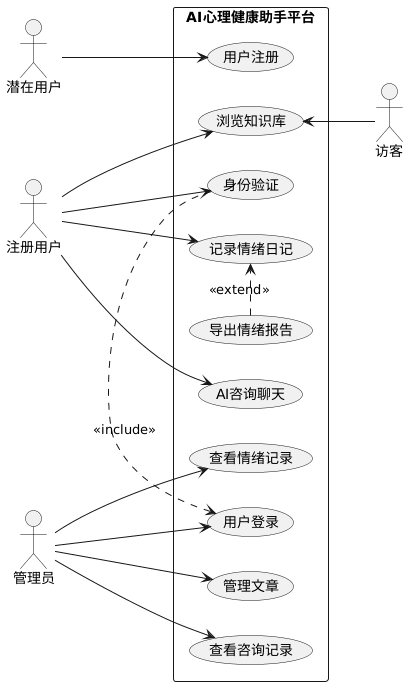
\includegraphics[width=0.7\textwidth]{plantuml.png}
    \caption{用例图}
\end{figure}


\section{附录 B：权限矩阵}
\begin{tabular}{|c|c|c|c|}
    \hline
    功能 & 访客 & 注册用户 & 管理员 \\
    \hline
    浏览首页 & ✓ & ✓ & ✓ \\
    用户注册 & ✓ & — & — \\
    用户登录 & ✓ & ✓ & ✓ \\
    AI咨询 & — & ✓ & ✓ \\
    情绪日记 & — & ✓ & ✓ \\
    浏览知识库 & ✓ & ✓ & ✓ \\
    管理文章 & — & — & ✓ \\
    查看咨询记录 & — & — & ✓ \\
    查看情绪记录 & — & — & ✓ \\
    \hline
\end{tabular}

\section{附录 C：优先级说明}
\begin{tabular}{|c|c|c|c|}
    \hline
    优先级 & 说明 & 包含用例 \\
    \hline
    高 & 核心功能 & UC1、UC2、UC3、UC4 \\
    中 & 重要功能 & UC5、UC6、UC7、UC8 \\
    \hline
\end{tabular}

